\section{Background}
\label{kvdirect:sec:background}


\egg{
\subsection{The Road to High Performance KVS}

Building a high performance KVS is a non-trivial exercise of optimizing various software and hardware components in a computer system. The rich literature on KVS performance optimizations can give us a glimpse of software and hardware evolution in recent years.
Early works on distributed in-memory KVS such as Memcached~\cite{fitzpatrick2004distributed} uses OS locks for multi-core synchronization and TCP/IP networking stack for communication. Since then, optimizations have been made on multiple fronts to remove bottlenecks in various parts of the system.


\subsubsection{Synchronization cost}
\label{kvdirect:sec:CoreSynchronizationCost}
Synchronization is needed in multi-threaded KVS implementation since multiple clients might access the same keys concurrently. For example, when two clients make atomic increments to a single key, the value needs to reflect both increments.

To reduce synchronization cost, Masstree~\cite{mao2012cache}, MemC3~\cite{fan2013memc3} and libcuckoo~\cite{li2014algorithmic} optimize caching, hashing and memory allocation algorithms, and replace permissive kernel locks with optimistic version-based locks.
MICA~\cite{lim2014mica, li2016full} takes a further step to completely avoid synchronization by partitioning the hash table to each core so that each core serves an exclusive portion of the hash table.
This approach, however, may introduce core imbalance for long-tail access patterns with a few extremely popular keys~\cite{li2016full}.

\subsubsection{Networking overhead}
\label{kvdirect:sec:ReduceNetworkingOverhead}

In a KVS where computation to communication ratio is low, a significant portion of CPU cycles is spent in the kernel networking stack, including protocol handling, memory copy, system call and multi-core synchronization~\cite{peter2016arrakis}.
Furthermore, the kernel network stack adds hundreds of microseconds latency~\cite{ousterhout2015ramcloud}, which greatly impacts response time.
and complicates latency-hiding programming of applications that require multiple round-trips to the KVS.

Extensive research have been done to reduce network communication cost and improve end-to-end latency.
One line of work proposes the KVS server software communicate directly with NICs by polling while bypassing the kernel~\cite{rizzo2012netmap, intel2014data}; packets are processed by a lightweight network stack in user space~\cite{jeong2014mtcp, marinos2014network}.
Chronos~\cite{kapoor2012chronos}, RAMCloud~\cite{ousterhout2010case, ousterhout2015ramcloud} and MICA~\cite{lim2014mica,li2016full} leverage this approach to achieve high throughput (\approx5 million KV operations per second (op/s) per core) and low latency (microsecond-scale) by reducing networking overhead.

The other line of work leverage two-sided RDMA~\cite{infiniband2000infiniband} as an RPC mechanism between KVS client and server.
RDMA is a hardware-based transport that almost completely removes the CPU overhead of networking.
KVS systems such as HERD~\cite{kalia2014using, kalia2016design} achieve per-core throughput and end-to-end latency comparable or superior to the first line of work, but the overall throughput per server largely depends on the processing capacity of RDMA NIC~\cite{kalia2016design}.

\subsubsection{Throughput bottleneck of CPU}
\label{kvdirect:sec:CPU-KV-Bottleneck}
When pushed to the limit, in high performance KVS systems the throughput bottleneck can be attributed to the computation in KV operation and the latency in random memory access. KVS needs to spend CPU cycles for key comparison and hash slot computation. Moreover, KVS hash table is orders of magnitude larger than the CPU cache, therefore the memory access latency is dominated by cache miss latency for practical access patterns.

By our measurement, a 64-byte random read latency for a contemporary computer (Sec.~\ref{kvdirect:sec:evaluation-setup}) is \approx110~ns. A CPU core can issue several memory access instructions concurrently when they fall in the instruction window, limited by the number of load-store units in a core (measured to be 3\approx4 in our CPU)~\cite{gharachorloo1992hiding, han2010packetshader, zhang2015mega}. In our CPU, we measure a max throughput of 29.3M random 64B access per second per core. On the other hand, an operation to access 64-byte KV pair typically requires \approx100ns computation or \approx500 instructions, which is too large to fit in the instruction window (measured to be 100\approx200). When interleaved with computation, the performance a CPU core degrades to only 5.5 MOps. An optimization is to batch memory accesses in a KV store by clustering the computation for several operations together before issuing the memory access all at once~\cite{li2016full, narula2014phase}. This improves the per-core throughput to 7.9 MOps in our CPU, which is still far less than the throughput of the host DRAM. 
}

\begin{comment}
When pushed to the limit, in high performance KVS systems the throughput bottleneck can be attributed to the computation in KV operation and the latency in random memory access. This is actually the bottleneck we want to remove in our design and we discuss the issue here in more detail. 

KVS needs to spend CPU cycles for key comparison and hash slot computation. Moreover, KVS hash table is orders of magnitude larger than the CPU cache, therefore the memory access latency is dominated by cache miss latency for practical access patterns.

\begin{figure}[t]
\centering
\subfloat[Single core.\label{kvdirect:fig:cpu-mem-single}]
{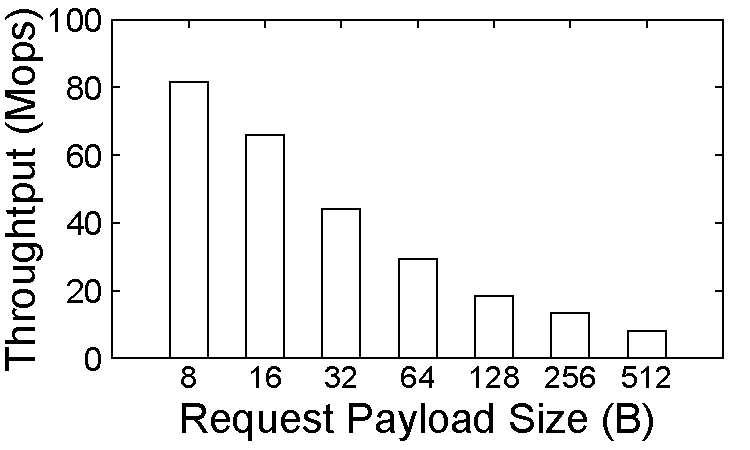
\includegraphics[width=.25\textwidth,page=1]{cpu_random_mem_single_core.pdf}}
\subfloat[Multiple cores.\label{kvdirect:fig:cpu-mem-multi}]
{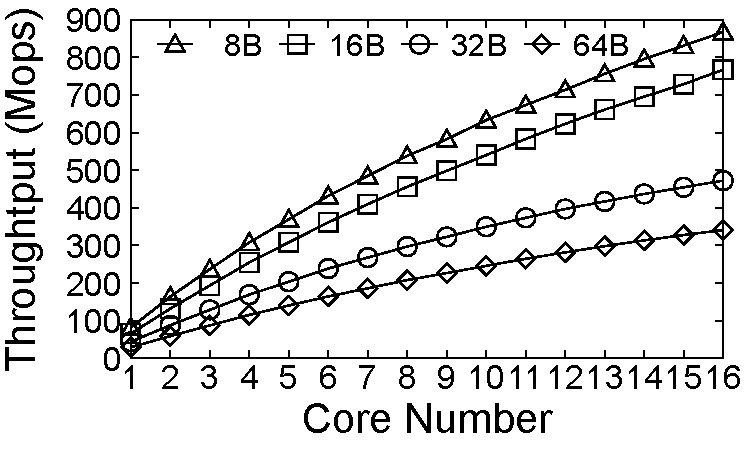
\includegraphics[width=.25\textwidth,page=1]{cpu_random_mem_multi_core.pdf}}
\caption{CPU random memory access performance.}
\label{kvdirect:fig:cpu-mem}
\end{figure}

The latency for CPU to access DRAM on the same NUMA node, \ie cache miss latency, is 80\approx90 nanoseconds on our platform (measured with~\cite{intelmemaccess}, hardware details in sec. \ref{kvdirect:sec:implementation}).
For 64-byte access granularity, the random read latency including data copy is \approx110~ns.
This latency can be partially hidden by the out-of-order execution engine in modern CPUs, which can issue a few memory accesses in parallel.
However, the parallelism is limited by two factors: the number of load-store units (LSUs) per core~\emph{k} (measured to be 3\approx4 on our CPU) and the instruction window size~\emph{W} (measured to be 100\approx200 instructions on our CPU)~\cite{gharachorloo1992hiding, han2010packetshader, zhang2015mega}. When there are enough memory operations in the instruction window, \emph{k} of them can be issued simultaneously. 

\begin{table}[htbp]
\footnotesize
\centering
\label{kvdirect:tab:tput-unroll}
\begin{tabular}{|c|c|c|c|c|c|c|}
\hline
\multirow{2}{*}{Size (B)} & \multirow{2}{*}{CalcOnly} & \multirow{2}{*}{MemOnly} & \multicolumn{4}{c|}{Calc + Mem (Batch Factor)} \\\cline{4-7} 
  &  & & 1 & 2 & 3 & 4 \\\hline
32 & 24.1 & 44.0 & 7.5 & 11.1 & 13.1 & 14.1 \\\hline
64 & 11.1 & 29.3 & 5.5 & 6.7 & 7.6 & 7.9 \\\hline
128 & 5.4 & 18.3 & 3.5 & 4.1 & 4.3 & 4.1 \\\hline
256 & 2.7 & 13.2 & 2.1 & 2.2 & 2.2 & 2.1 \\\hline
512 & 1.3 & 8.2 & 1.2 & 1.1 & 1.2 & 1.1 \\\hline
\end{tabular}
\caption{Throughput (M op/s) under different workload and payload sizes of memory access.}
\label{kvdirect:tab:kv-cpu-throughput}
\end{table}

Figure~\ref{kvdirect:fig:cpu-mem} shows random memory access performances of a multicore CPU. It shows that a modern CPU core can provide fairly high random memory access throughput (27M~op/s or 1.7~GB/s for 64B granularity). Moreover, memory throughput scales linearly with number of CPU cores, indicating that the DDR main memory is not a bottleneck.

However, in a KV store memory access is interleaved with computation for hash slot calculation and key comparison. An operation to access a 64-byte KV pair typically requires \approx100 ns computation or \approx500 instructions, which is far larger than the instruction window size.
Consequently, when the random memory access instructions for different keys are separated by computation, the second DRAM access is too far to fit in the same instruction window with the first DRAM access and cannot be issued in parallel.

One can batch memory accesses in a KV store, i.e. clustering the computation for several operations together before issuing the memory access all at once~\cite{li2016full, narula2014phase}.
Table~\ref{kvdirect:tab:kv-cpu-throughput} depicts the measured per-core hash table throughput under different KV sizes and batch sizes, assuming the KV is inlined in hash table and each KV operation requires one non-cached memory access.
The results fit the following formulas within 10\% error:
\begin{equation}
%\small
\frac{1}{RandAccessThroughput} = \frac{MemLatency}{Parallelism}
\end{equation}
\begin{equation}
%\small \frac{1}{KVThroughput} = ComputeTime + \frac{MemLatency}{min(BatchSz, Parallelism)}
\begin{aligned}
\frac{1}{KVopThroughput} = & ComputationTime + \\
      & \frac{MemLatency}{min(BatchSize, Parallelism)}
\end{aligned}
\end{equation}
This indicates that when interleaved with computation, the performance of CPU degrades significantly. In the extreme case, even if the instruction window size or memory fetch parallelism goes to infinity, the per-core KV operation throughput would still be bounded by computation (\approx10M~op/s), 10\approx20x slower than a single DDR channel.
\end{comment}

\egg{
\subsection{Domain-Specific Architectures for KVS}

Ten years ago, processor frequency scaling was over and people turned to multi-core and concurrency~\cite{sutter2005free}.
Nowadays, CMOS feature-size reduction is getting more and more difficult, which implies that multi-core scaling is also over. People are turning to domain-specific architectures (DSAs)~\cite{esmaeilzadeh2013power} for better performance. Several such DSAs have been used to improve KVS performances. 

\egg{
For computation, DSAs such as GPU, 
FPGA~\cite{putnam2014programmable, caulfield2016cloud} and ASIC~\cite{liu2016cambricon, tpu} have been quickly accepted by the market.
For networking, DSAs are also deployed at scale in datacenters, such as RDMA/RoCE NICs~\cite{mellanoxrdma}, programmable NICs~\cite{greenberg2015sdn, li2016clicknp} and programmable switches~\cite{bosshart2013forwarding}.
}

\subsubsection{One-sided RDMA}

Due to high overhead in CPU network processing, DSAs to accelerate networking, such as RDMA/RoCE NICs~\cite{mellanoxrdma}, are deployed at scale in datacenters. High performance KVS systems can leverage RDMA capable hardware. One approach is to accelerate RPC with \textit{two-sided} verbs in RDMA/RoCE NICs (section \ref{kvdirect:sec:ReduceNetworkingOverhead}, Figure~\ref{kvdirect:fig:memaccess-a}).
By doing so, the KV performance is bounded by CPU (section \ref{kvdirect:sec:CPU-KV-Bottleneck}).

A significantly different approach is to leverage \textit{one-sided} RDMA to access remote memory via the NIC on the client and bypass the CPU on the server, as shown in Figure~\ref{kvdirect:fig:memaccess-b}.
In this approach, KV computation and synchronization are handled by the client CPU, therefore making the KV server very light-weight and high performance.
Despite the high message rate (8M\approx150M~op/s~\cite{kalia2016design}) provided by RDMA NICs, it is challenging to find an efficient match between RDMA primitives and key-value operations.
For a write (PUT or atomic) operation, multiple network round-trips and memory accesses may be required to handle hash conflicts, memory allocation and fetch/save non-inline data.
RDMA does not support transactions. Clients must synchronize with each other to ensure consistency by either using RDMA atomics or distributed atomic broadcast~\cite{szepesi2014designing}, both incurring communication overhead and synchronization latency~\cite{mitchell2013using, dragojevic2014farm}.
As a consequence, most RDMA-based KVS, \eg, Pilaf~\cite{mitchell2013using}, FaRM~\cite{dragojevic2014farm} and HERD~\cite{kalia2014using} recommend using one-sided RDMA for GET operations only. For PUT operations, they fall back to two-sided RDMA as RPC and let the remote CPU do the actual work. Throughput of write-intensive workload is still bottlenecked by CPU cores.

In addition to the mismatch between RDMA primitives and KV operations, implementation of commodity RDMA NICs also constrain KV throughput. For example, RDMA NICs hold a lock for atomic operations when a PCIe DMA to the same memory address is in flight, which bounds RDMA atomics throughput to \approx2M~op/s~\cite{kalia2016design}.

\subsubsection{Highly parallel architectures}

Highly parallel architectures such as many-core processors~\cite{berezecki2011many}, GPGPU~\cite{zhang2015mega}.

\subsubsection{FPGA}

FPGA~\cite{istvan2013flexible, chalamalasetti2013fpga, maohardware, lavasani2014fpga, istvan2015hash, istvan2016consensus, kvs-openpower, istvan2015hash, sidler2015scalable, blott2015scaling} have been explored to overcome the limited parallelism of CPU in accessing DRAM.
Compared to general-purpose processors, FPGA has more flexible pipeline parallelism and can be specialized for the key-value store application.
Compared to RDMA, FPGA can support key-value operation primitives directly, as well as specializing network packet format and PCIe DMA operations to use network and PCIe bandwidth efficiently.
Compared to GPGPU, FPGA is more power-efficient and has lower latency.

In recent years, FPGA is becoming cost-effective and is getting deployed at scale in datacenters~\cite{putnam2014programmable, caulfield2016cloud}. Its programmability has been greatly improved~\cite{li2016clicknp}.
Most existing work store the entire hash table inside the on-board DRAM, which is often quite limiting (typically on the order of 4\approx16~GiB), while the host DRAM is often large (on the order of 100\approx500~GiB).
KV-Direct follows this line of work, while leveraging host DRAM for KV storage, as depicted in Figure~\ref{kvdirect:fig:memaccess-c}.

KV-Direct leverages a programmable NIC with large-scale deployments in datacenters.
The programmable NIC is composed of two parts: a traditional RDMA NIC plus a field-programmable gate array (FPGA).
There has been research on leveraging the reconfigurability of the NIC for network processing, \eg, network virtualization~\cite{greenberg2015sdn, vfp} and network functions~\cite{li2016clicknp}.
KV-Direct extends the application of programmable NICs to a novel area: key-value stores.
}

\subsection{Workload Shift in KVS}
\label{kvdirect:sec:workload-shift}

\textbf{讨论 serverless computing 中的 shared storage}

Historically, KVS such as Memcached~\cite{fitzpatrick2004distributed} gained popularity as an object caching system for web services.
In the era of in-memory computation, KVS goes beyond caching and becomes an infrastructure service to store shared data structure in a distributed system.
Many data structures can be expressed in a key-value hash table, \eg, data indexes in NoSQL databases~\cite{chang2008bigtable}, model parameters in machine learning~\cite{li2014scaling}, nodes and edges in graph computing~\cite{shao2013trinity, xiao17tux2} and sequencers in distributed synchronization~\cite{kalia2016design,eris}.

The workload shifts from object cache to generic data structure store implies several design goals for KVS.

\textbf{High batch throughput for small KV.}
In-memory computations typically access small key-value pairs in large batches, \eg, sparse parameters in linear regression~\cite{li2014algorithmic, xiao17tux2} or all neighbor nodes in graph traversal~\cite{shao2013trinity}, therefore a KVS should be able to benefit from batching and pipelining.
%If the throughput of remote key-value access is comparable to accessing a local hash table, distributed computation on shared memory could be easier to scale linearly.

\textbf{Predictable low latency.}
For many data-parallel computation tasks, the latency of an iteration is determined by the slowest operations~\cite{ousterhout2015ramcloud}. Therefore, it is important to control the tail latency of KVS. CPU based implementations often have large fluctuations under heavy load due to scheduling irregularities and inflated buffering.
%CPU-based designs may need to trade-off latency and throughput by adjusting batch size~\cite{li2016full}, while hardware-accelerated designs can leverage pipelining to boost throughput without sacrificing latency~\cite{kalia2016design}.
%Additionally, CPU processing time may have large fluctuations under high load due to scheduling irregularities, while hardware pipelines often have stable latency~\cite{li2016clicknp}.

\textbf{High efficiency under write-intensive workload.}
For cache workloads, KVS often has much more reads than writes~\cite{atikoglu2012workload}, but it is no longer the case for distributed computation workloads
such as graph computation~\cite{page1999pagerank}, parameter servers~\cite{li2014scaling}.
%For PageRank computation in a graph~\cite{page1999pagerank} or gradient descent in parameter servers~\cite{li2014scaling}, each node or parameter is read and written once per iteration, and the KVS would serve an equal number of GET and PUT operations.
%Sequencers~\cite{kalia2016design} require atomic increment operations and no read-only operations.
These workloads favor hash table structures that can handle both read and write operations efficiently.


\textbf{Fast atomic operations.}
Atomic operations on several extremely popular keys appear in applications such as centralized schedulers~\cite{perry2014fastpass}, sequencers~\cite{kalia2016design,eris}, counters~\cite{zhu2015packet} and short-term values in web applications~\cite{atikoglu2012workload}.
This requires high throughput on single-key atomics.
%CPU-based KVS atomics is bottlenecked by either core contention or per-core throughput~\cite{li2016full}, and atomics based on one-sided RDMA is bottlenecked by PCIe latency~\cite{kalia2016design}.

\textbf{Support vector-type operations.}
Machine learning and graph computing workloads~\cite{li2014scaling,shao2013trinity,xiao17tux2} often require operating on every element in a vector,
\eg, incrementing every element in a vector with a scalar or reducing a vector into the sum of its elements.
KVS without vector support requires the client to either issue one KVS operation per element, or retrieve the vector back to the client and perform the operation.
Supporting vector data type and operations in KVS can greatly reduce network communication and CPU computation overhead.


\subsection{Achilles' Heel of High-Performance KVS Systems}
\label{kvdirect:sec:state-of-the-art-kvs}

Building a high performance KVS is a non-trivial exercise of optimizing various software and hardware components in a computer system.
Characterized by where the KV processing takes place, state-of-the-art high-performance KVS systems basically falls into three categories:
on the CPU of KVS server
%~\cite{mao2012cache,fan2013memc3,li2014algorithmic,ousterhout2010case, ousterhout2015ramcloud, kapoor2012chronos, lim2014mica,li2016full,kalia2014using, kalia2016design}
(Figure~\ref{kvdirect:fig:memaccess-a}),
on KVS clients
%~\cite{mitchell2013using,szepesi2014designing,dragojevic2014farm,kalia2014using}
(Figure~\ref{kvdirect:fig:memaccess-b})
or on a hardware accelerator
%~\cite{zhang2015mega,berezecki2011many,liang16fpl,blott13hotcloud,lavasani2014fpga,chalamalasetti2013fpga}
(Figure~\ref{kvdirect:fig:memaccess-c}).

When pushed to the limit, in high performance KVS systems the throughput bottleneck can be attributed to the computation in KV operation and the latency in random memory access.
CPU-based KVS needs to spend CPU cycles for key comparison and hash slot computation.
Moreover, KVS hash table is orders of magnitude larger than the CPU cache, therefore the memory access latency is dominated by cache miss latency for practical access patterns.

By our measurement, a 64-byte random read latency for a contemporary computer is \approx110~ns. A CPU core can issue several memory access instructions concurrently when they fall in the instruction window, limited by the number of load-store units in a core (measured to be 3\approx4 in our CPU)~\cite{gharachorloo1992hiding, han2010packetshader, zhang2015mega}. In our CPU, we measure a max throughput of 29.3~M random 64B access per second per core. On the other hand, an operation to access 64-byte KV pair typically requires \approx100~ns computation or \approx500 instructions, which is too large to fit in the instruction window (measured to be 100\approx200). When interleaved with computation, the performance of a CPU core degrades to only 5.5~M KV operations per second (Mops). An optimization is to batch memory accesses in a KV store by clustering the computation for several operations together before issuing the memory access all at once~\cite{li2016full, narula2014phase}. This improves the per-core throughput to 7.9~MOps in our CPU, which is still far less than the random 64B throughput of host DRAM.

Observing the limited capacity of CPU in KV processing, recent work~\cite{mitchell2013using,szepesi2014designing,dragojevic2014farm} leverage one-sided RDMA to offload KV processing to clients and effectively using the KVS server as a shared memory pool.
Despite the high message rate (8\approx150~Mops~\cite{kalia2016design}) provided by RDMA NICs, it is challenging to find an efficient match between RDMA primitives and key-value operations.
For a write (PUT or atomic) operation, multiple network round-trips and multiple memory accesses may be required to query the hash index, handle hash collisions and allocate variable-size memory.
RDMA does not support transactions. Clients must synchronize with each other to ensure consistency using RDMA atomics or distributed atomic broadcast~\cite{szepesi2014designing}, both incurring communication overhead and synchronization latency~\cite{mitchell2013using, dragojevic2014farm}.
Therefore, most RDMA-based KVS~\cite{mitchell2013using,dragojevic2014farm,kalia2014using} recommend using one-sided RDMA for GET operations only. For PUT operations, they fall back to the server CPU. The throughput of write-intensive workload is still bottlenecked by CPU cores.

\subsection{Programmable NIC with FPGA}
\label{kvdirect:sec:programmable-nic}

\begin{figure}[t]
\centering
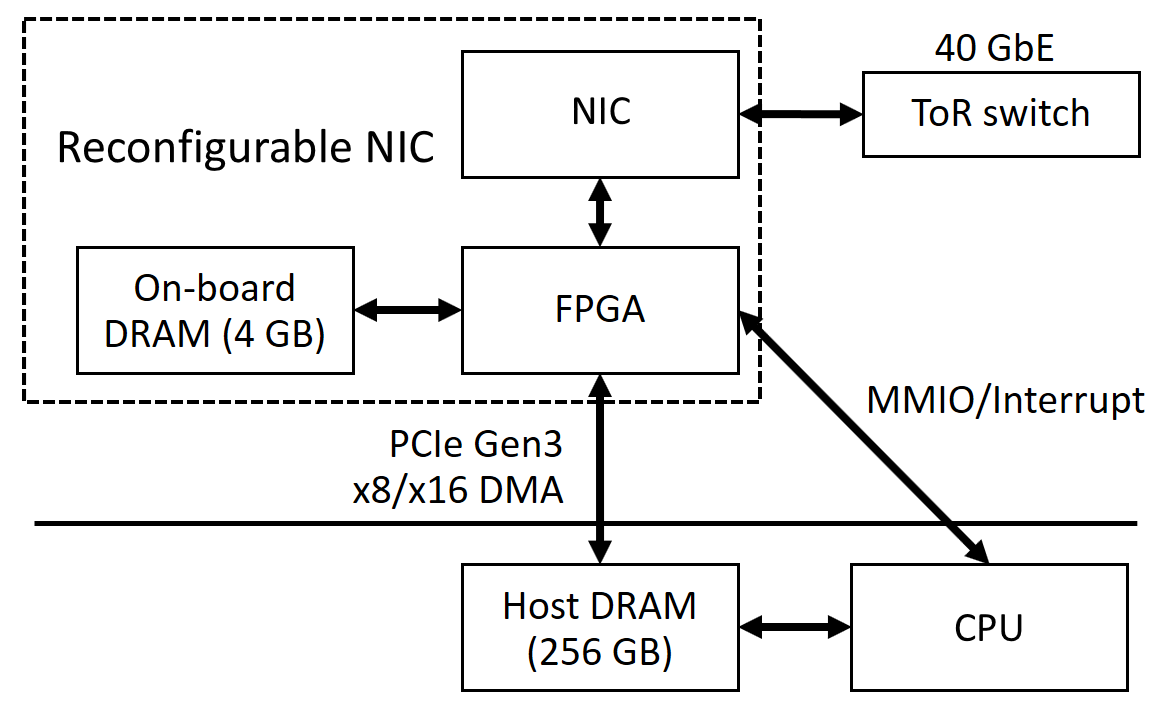
\includegraphics[width=0.6\textwidth]{sys_architecture.PNG}
\caption{Programmable NIC with FPGA.}
\label{kvdirect:fig:kvdirect-arch}

\end{figure}

Ten years ago, processor frequency scaling slowed down and people turned to multi-core and concurrency~\cite{sutter2005free}.
Nowadays, power ceiling implies that multi-core scaling has also met difficulties~\cite{esmaeilzadeh2013power}.
People are now turning to domain-specific architectures (DSAs) for better performance.

%On the spectrum of hardware programmability and performance, general-purpose processors lie on the programmability end, while application-specific integrated circuits (ASICs) lie on the performance end.
%Field-programmable gate array (FPGA) is an architecture between the two extremes, providing both programmability and performance~\cite{bacon2013fpga}.
%As its name indicates, FPGA is a sea of gates.
%Millions of reconfigurable gates and thousands of small block RAMs (BRAMs) provide massive parallelism to build thousands of ``cores'' running simultaneously, and more importantly, customized interconnections among the ``cores'' and BRAMs specializing communication and synchronization for a certain application.
%Consequently, for applications with sufficient bit-level and task-level parallelism, FPGAs provide not only high throughput and power efficiency, but also low and predictable latency.

Due to the increasing mismatch of network speed and CPU network processing capacity, programmable NICs with FPGA~\cite{vfp,greenberg2015sdn,li2016clicknp,caulfield2016cloud} now witness large-scale deployment in datacenters.
As shown in Figure~\ref{kvdirect:fig:kvdirect-arch}, the heart of the programmable NIC we use is an FPGA, with an embedded NIC chip to connect to the network.
Programmable NICs typically come with on-board DRAM as packet buffers and runtime memory for NIC firmware~\cite{li2016clicknp}, but the DRAM is typically not large enough to hold the entire key-value store.

\subsection{Challenges for Remote Direct Key-Value Access}
\label{kvdirect:sec:challenge}

\begin{figure}[t]
\centering
\subfloat[Throughput.\label{kvdirect:fig:dma-tput}]
{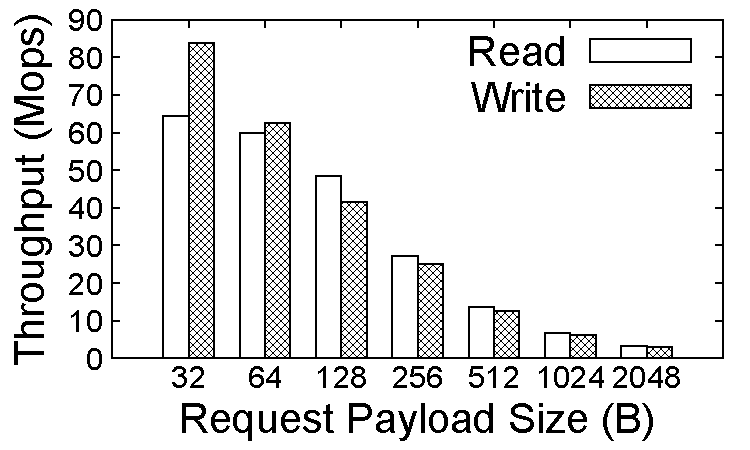
\includegraphics[width=.5\textwidth,page=1]{pcie_bw.pdf}}
\subfloat[DMA Read Latency.\label{kvdirect:fig:dma-lat}]
{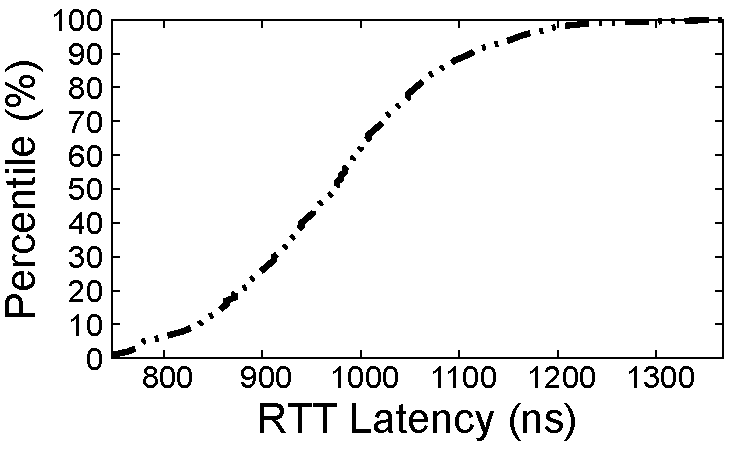
\includegraphics[width=.5\textwidth,page=1]{pcie_latency.pdf}}
\caption{PCIe random DMA performance.}
\label{kvdirect:fig:dma-perf}

\end{figure}

KV-Direct moves KV processing from the CPU to the programmable NIC in the server (Figure~\ref{kvdirect:fig:memaccess-c}).
Same as RDMA, the KV-Direct NIC accesses host memory via PCIe. PCIe is a packet switched network with \approx500~ns round-trip latency and 7.87~GB/s theoretical bandwidth per Gen3 x8 endpoint.
On the latency side, for our programmable NIC, the cached PCIe DMA read latency is 800~ns due to additional processing delay in FPGA.
For random non-cached DMA read, there is an additional 250~ns average latency (Figure~\ref{kvdirect:fig:dma-lat}) due to DRAM access, DRAM refresh and PCIe response reordering in PCIe DMA engine.
On the throughput side, each DMA read or write operation needs a PCIe transport-layer packet (TLP) with 26-byte header and padding for 64-bit addressing.
For a PCIe Gen3 x8 NIC to access host memory in 64-byte granularity, the theoretical throughput is therefore 5.6~GB/s, or 87~Mops.

To saturate PCIe Gen3 x8 with 64-byte DMA requests, 92 concurrent DMA requests are needed considering our latency of 1050~ns.
In practice, two factors further limit the concurrency of DMA requests.
First, PCIe credit-based flow control constrains the number of in-flight requests for each DMA type. The PCIe root complex in our server advertises 88 TLP posted header credits for DMA write and 84 TLP non-posted header credits for DMA read.
Second, DMA read requires assigning a unique PCIe tag to identify DMA responses which may come out of order.
The DMA engine in our FPGA only support 64 PCIe tags, further limiting our DMA read concurrency to 64 requests, which renders a throughput of 60~Mops as shown in Figure~\ref{kvdirect:fig:dma-tput}.
On the other hand, with 40~Gbps network and 64-byte KV pairs, the throughput ceiling is 78~Mops with client-side batching.
In order to saturate the network with GET operations, the KVS on NIC must make full use of PCIe bandwidth and achieve close to one average memory access per GET.
This boils down to three challenges:

\textbf{Minimize DMA requests per KV operation.}
Hash table and memory allocation are two major components in KVS that require random memory access.
Previous works propose hash tables~\cite{dragojevic2014farm, breslow2016horton} with close to 1 memory access per GET operation even under high load factors.
However, under higher than 50\% load factor, these tables need multiple memory accesses per PUT operation on average with large variance.
This not only consumes PCIe throughput, but also leads to latency variations for write-intensive workloads.

In addition to hash table lookup, dynamic memory allocation is required to store variable-length KVs that cannot be inlined in the hash table.
Minimizing hash table lookups per KV operation and memory accesses per memory allocation is essential for matching PCIe and network throughput under write-intensive, small-KV workloads.

\textbf{Hide PCIe latency while maintaining consistency.}
An efficient KVS on NIC must pipeline KV operations and DMA requests to hide the PCIe latency.
However, KV operations may have dependencies.
A GET following PUT on a same key needs to return the updated value.
%Two adjacent atomic add operations needs to wait for the first to finish before executing the second.
This requires tracking KV operations being processed and stall the pipeline on data hazard, or better, design an out-of-order executor to resolve data dependency without explicitly stalling the pipeline.


\textbf{Dispatch load between NIC DRAM and host memory.}
%Currently the DRAM is underutilized both in terms of space and throughput.
An obvious idea is to use the DRAM on NIC as a cache for host memory, but in our NIC, the DRAM throughput (12.8~GB/s) is on par with the achievable throughput (13.2~GB/s) of two PCIe Gen3 x8 endpoints.
It is more desirable to distribute memory access between DRAM and host memory in order to utilize both of their bandwidths.
However, the on-board DRAM is small (4~GiB) compared to the host memory (64~GiB), calling for a hybrid caching and load-dispatching approach.

In the following, we will present KV-Direct, a novel FPGA-based key-value store that satisfies all aforementioned goals and describe how we address the challenges.
